\documentclass[11pt,letterpaper]{article}

\usepackage[margin=1in]{geometry}
\usepackage[T1]{fontenc}
\usepackage[utf8]{inputenc}
\usepackage{lmodern}
\usepackage{amsmath,amssymb,mathtools}
\usepackage{booktabs}
\usepackage{enumitem}
\usepackage{parskip}
\usepackage[dvipsnames]{xcolor}
\usepackage[unicode=true]{hyperref}
\usepackage{fancyhdr}
\usepackage[most]{tcolorbox}
\usepackage{tikz}
\usetikzlibrary{arrows.meta,positioning,calc}

\hypersetup{
  colorlinks=true,
  linkcolor=MidnightBlue,
  urlcolor=MidnightBlue
}

\pagestyle{fancy}
\fancyhf{}
\fancyhead[L]{\small Hessian and Sharpness Explainer}
\fancyhead[R]{\small \thepage}

\newtcolorbox{keyidea}{
  colback=blue!3,
  colframe=MidnightBlue!70!black,
  title=\textbf{Key Idea}
}

\newtcolorbox{takeaway}{
  colback=green!3,
  colframe=ForestGreen!60!black,
  title=\textbf{Practical Takeaway}
}

\newtcolorbox{warningbox}{
  colback=red!3,
  colframe=BrickRed!60!black,
  title=\textbf{Important Caveat}
}

\newcommand{\R}{\mathbb{R}}
\newcommand{\E}{\mathbb{E}}
\newcommand{\tr}{\operatorname{tr}}
\newcommand{\diag}{\operatorname{diag}}
\newcommand{\sign}{\operatorname{sign}}
\newcommand{\norm}[1]{\left\lVert #1 \right\rVert}
\newcommand{\abs}[1]{\left\lvert #1 \right\rvert}
\newcommand{\ip}[2]{\left\langle #1, #2 \right\rangle}

\tikzset{
  flowbox/.style={
    draw=MidnightBlue!70!black,
    fill=blue!4,
    rounded corners=2pt,
    align=center,
    font=\small,
    inner sep=5pt,
    minimum height=0.8cm
  },
  sharpbox/.style={
    draw=ForestGreen!60!black,
    fill=green!4,
    rounded corners=2pt,
    align=center,
    font=\small,
    inner sep=5pt,
    minimum height=0.8cm
  },
  trbox/.style={
    draw=BrickRed!65!black,
    fill=red!4,
    rounded corners=2pt,
    align=center,
    font=\small,
    inner sep=5pt,
    minimum height=0.8cm
  },
  flowarrow/.style={-{Stealth[length=2.5mm]}, thick}
}

\title{\textbf{How Hessian and Sharpness Work in the Raman-Suppression Codebase}\\[4pt]
\large A code-grounded pedagogical note}
\author{Prepared from the repository state on 2026-04-23}
\date{\today}

\begin{document}
\maketitle

\begin{abstract}
This note explains, in a code-grounded and pedagogical way, what the
\emph{Hessian} and \emph{sharpness} mean in this repository, how they are
computed, when each one is used, and how they relate to the base Raman
suppression optimization pipeline.

The short version is:
\begin{enumerate}[leftmargin=*]
  \item The code's \textbf{Hessian machinery} is mainly a \emph{diagnostic}
  tool. It is used to probe local curvature of the physical loss near an
  already-optimized phase, mainly through Hessian-vector products and
  eigenvalue calculations.
  \item The code's \textbf{sharpness machinery} is mainly an
  \emph{optimization regularizer}. It adds a stochastic estimate of local
  curvature to the objective so that the optimizer prefers flatter, more robust
  basins rather than merely deeper ones.
\end{enumerate}

These two mechanisms are related, but they are not the same thing. The
Hessian path tries to understand the full local geometry. The sharpness path
uses a cheaper trace-like summary of that geometry inside the objective.

One caveat is important: the default production optimizer is L-BFGS and does
not use Hessian/Newton steps, but the repository also contains a separate
research trust-region optimizer that uses finite-difference Hessian-vector
products during optimization.
\end{abstract}

\section{Roadmap}

The relevant implementation lives in these main files:
\begin{enumerate}[leftmargin=*]
  \item {\footnotesize\path{scripts/lib/raman_optimization.jl}}\\
  Base physical cost and adjoint gradient.
  \item {\footnotesize\path{scripts/research/phases/phase13/hvp.jl}}\\
  Matrix-free finite-difference Hessian-vector products.
  \item {\footnotesize\path{scripts/research/phases/phase13/hessian_eigspec.jl}}\\
  Eigenspectrum extraction from those HVPs.
  \item {\footnotesize\path{scripts/lib/sharpness_optimization.jl}}\\
  Sharpness-aware objective and optimizer wrapper.
  \item {\footnotesize\path{scripts/research/trust_region/trust_region_optimize.jl}}\\
  Separate Newton-style trust-region research optimizer that uses HVPs inside
  the optimization loop.
\end{enumerate}

\section{The Three Places Curvature Appears}

The easiest way to avoid confusion is to separate three code paths:

\begin{figure}[htbp]
\centering
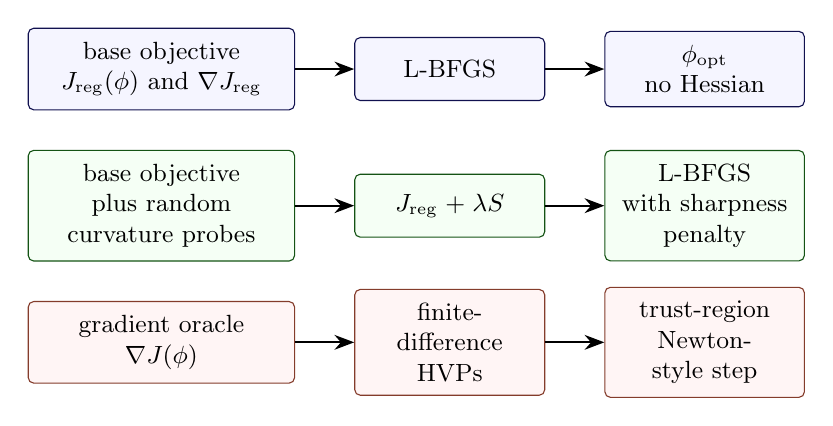
\begin{tikzpicture}[node distance=0.5cm and 0.75cm]
  \node[flowbox,text width=0.25\textwidth] (base1) {base objective\\$J_{\mathrm{reg}}(\phi)$ and $\nabla J_{\mathrm{reg}}$};
  \node[flowbox,right=of base1,text width=0.17\textwidth] (base2) {L-BFGS};
  \node[flowbox,right=of base2,text width=0.18\textwidth] (base3) {$\phi_{\mathrm{opt}}$\\no Hessian};
  \draw[flowarrow] (base1) -- (base2);
  \draw[flowarrow] (base2) -- (base3);

  \node[sharpbox,below=of base1,text width=0.25\textwidth] (sharp1) {base objective\\plus random curvature probes};
  \node[sharpbox,right=of sharp1,text width=0.17\textwidth] (sharp2) {$J_{\mathrm{reg}}+\lambda S$};
  \node[sharpbox,right=of sharp2,text width=0.18\textwidth] (sharp3) {L-BFGS\\with sharpness penalty};
  \draw[flowarrow] (sharp1) -- (sharp2);
  \draw[flowarrow] (sharp2) -- (sharp3);

  \node[trbox,below=of sharp1,text width=0.25\textwidth] (tr1) {gradient oracle\\$\nabla J(\phi)$};
  \node[trbox,right=of tr1,text width=0.17\textwidth] (tr2) {finite-difference\\HVPs};
  \node[trbox,right=of tr2,text width=0.18\textwidth] (tr3) {trust-region\\Newton-style step};
  \draw[flowarrow] (tr1) -- (tr2);
  \draw[flowarrow] (tr2) -- (tr3);
\end{tikzpicture}
\caption{Three separate paths in the repo. The default optimizer is first-order L-BFGS. Sharpness modifies the objective but still usually uses L-BFGS. The trust-region research path uses HVPs as part of a Newton-style optimizer.}
\end{figure}

\begin{takeaway}
When someone says ``the Hessian code,'' ask which path they mean. In this
repository, Hessian-vector products are mostly diagnostic, sharpness is a
regularizer, and trust-region Newton is a separate research optimizer.
\end{takeaway}

\section{The Base Quantity Being Differentiated}

Everything starts from the same underlying function:
\[
J(\phi),
\]
where $\phi$ is the spectral phase applied to the input pulse.

In code, the base forward-adjoint computation is implemented in
\texttt{cost\_and\_gradient(...)} in
\path{scripts/lib/raman_optimization.jl}. The pipeline is:
\begin{enumerate}[leftmargin=*]
  \item apply the spectral phase to the input field,
  \item propagate the field through the fiber,
  \item evaluate the Raman-band cost at the output,
  \item solve the adjoint problem backward,
  \item apply the chain rule to get $\nabla_\phi J$.
\end{enumerate}

Schematically, the code computes
\[
\phi \longmapsto u_{\omega,0} e^{i\phi}
\longmapsto \text{fiber propagation}
\longmapsto J(\phi),
\]
and then returns both the scalar objective and its gradient with respect to
$\phi$.

\subsection{Regularized and log-scaled objective}

The code can optimize either a linear-scale objective or a dB-scaled one, and
it can add regularization terms such as GDD and boundary penalties. So the
actual optimized surface is often
\[
J_{\mathrm{reg}}(\phi)
= J_{\mathrm{physics}}(\phi)
  + \lambda_{\mathrm{gdd}} R_{\mathrm{gdd}}(\phi)
  + \lambda_{\mathrm{boundary}} R_{\mathrm{boundary}}(\phi),
\]
possibly followed by a log transform.

\begin{takeaway}
Whenever this note says ``Hessian'' or ``sharpness,'' it always means the
second-order geometry of \emph{whatever loss function the code is currently
using}. In some paths that is the plain linear physical loss. In other paths
that is the dB-scaled, regularized loss.
\end{takeaway}

\section{What the Hessian Means Here}

Mathematically, the Hessian is the matrix of second derivatives:
\[
H(\phi) = \nabla_\phi^2 J(\phi).
\]

If the gradient tells you the local slope, the Hessian tells you the local
curvature:
\begin{itemize}[leftmargin=*]
  \item positive curvature means ``bowl-shaped'' in that direction,
  \item negative curvature means ``saddle'' or ``downhill escape'' direction,
  \item near-zero curvature means ``flat'' direction.
\end{itemize}

For a perturbation $v$, the Hessian-vector product
\[
H(\phi)v
\]
tells you how the gradient changes if you move infinitesimally in direction
$v$.

\subsection{Why the code does not build the full Hessian by default}

The phase dimension is large. On production grids the optimization variable can
have thousands of components, so explicitly building the dense Hessian matrix
would be expensive in both time and memory.

Instead, the repo usually works \emph{matrix-free}: it computes
\[
v \mapsto H(\phi)v
\]
without ever forming the full matrix.

In plain language, that means the code knows how the Hessian acts on a vector,
without ever writing down every entry of the Hessian itself.

\section{How the Hessian-Vector Product is Computed}

The implementation in \path{scripts/research/phases/phase13/hvp.jl} uses a
central finite difference of the gradient:
\[
H(\phi)v
\;\approx\;
\frac{\nabla J(\phi + \varepsilon \hat v) - \nabla J(\phi - \varepsilon \hat v)}
     {2\varepsilon}\,\norm{v},
\qquad
\hat v = \frac{v}{\norm{v}}.
\]

\begin{figure}[htbp]
\centering
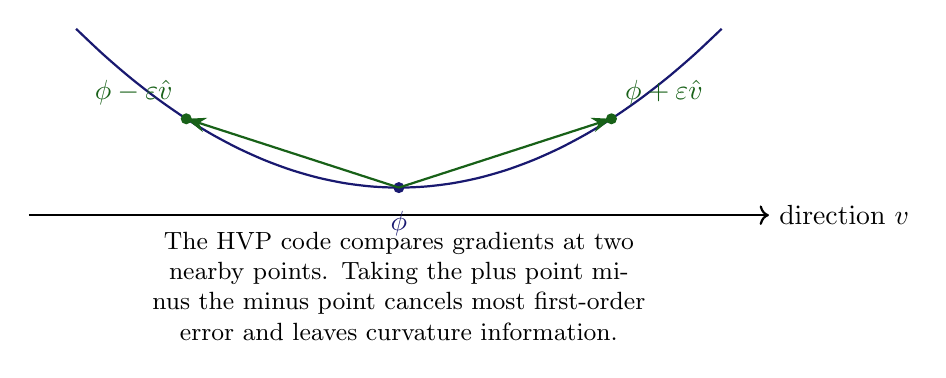
\begin{tikzpicture}[x=1cm,y=1cm]
  \draw[->,thick] (-4.7,0) -- (4.7,0) node[right] {direction $v$};
  \draw[MidnightBlue,thick,domain=-4.1:4.1,smooth,variable=\x]
    plot ({\x},{0.12*\x*\x + 0.35});
  \coordinate (center) at (0,0.35);
  \coordinate (minus) at (-2.7,1.224);
  \coordinate (plus) at (2.7,1.224);
  \fill[MidnightBlue] (center) circle (2pt) node[below=5pt] {$\phi$};
  \fill[ForestGreen!70!black] (minus) circle (2pt) node[above left=2pt] {$\phi-\varepsilon\hat v$};
  \fill[ForestGreen!70!black] (plus) circle (2pt) node[above right=2pt] {$\phi+\varepsilon\hat v$};
  \draw[flowarrow,ForestGreen!70!black] (center) -- (plus);
  \draw[flowarrow,ForestGreen!70!black] (center) -- (minus);
  \node[align=center,font=\small,text width=0.62\textwidth] at (0,-0.9)
    {The HVP code compares gradients at two nearby points. Taking the plus point minus the minus point cancels most first-order error and leaves curvature information.};
\end{tikzpicture}
\caption{Central finite difference picture for a Hessian-vector product.}
\end{figure}

\subsection{Why the direction is normalized}

The code first replaces $v$ by $\hat v = v/\norm{v}$, perturbs by a fixed
small step $\varepsilon \hat v$, then rescales by $\norm{v}$ at the end.

This is numerically important. Without normalization, a large-norm $v$ would
produce an enormous perturbation $\varepsilon v$, and a tiny-norm $v$ would
produce an almost invisible perturbation. The normalization makes the finite
difference step size controlled by $\varepsilon$, not by the arbitrary scale of
$v$.

\subsection{Cost of one HVP}

One HVP requires two gradient evaluations:
\begin{enumerate}[leftmargin=*]
  \item $\nabla J(\phi + \varepsilon \hat v)$,
  \item $\nabla J(\phi - \varepsilon \hat v)$.
\end{enumerate}

Since each gradient evaluation itself requires a forward solve plus an adjoint
solve, one HVP is already a nontrivial operation. That is another reason the
code prefers matrix-free methods.

\section{How the Hessian Eigenspectrum is Computed}

Once the code can apply $H$ to arbitrary vectors, it wraps that HVP in a
matrix-free linear operator and gives it to \texttt{Arpack.eigs}.

\subsection{What is extracted}

The eigenspectrum script computes:
\begin{itemize}[leftmargin=*]
  \item the biggest positive-curvature eigenvalues, using \texttt{:LR},
  \item the most negative or smallest eigenvalues, using \texttt{:SR}.
\end{itemize}

So it is not trying to recover the entire spectrum. It is trying to recover
the two most informative wings:
\begin{enumerate}[leftmargin=*]
  \item the stiff positive-curvature directions,
  \item the soft or negative-curvature directions.
\end{enumerate}

\subsection{Interpretation}

Suppose the code finds
\[
\lambda_{\max} > 0
\qquad\text{and}\qquad
\lambda_{\min} < 0.
\]
Then the point is \emph{indefinite}: in simpler words, it is not a true minimum.
It is a saddle, meaning some directions curve up while other directions curve
down.

That was the key Phase 13 geometry result: the canonical L-BFGS optima were not
true minima. They had negative-curvature directions that first-order L-BFGS was
not exploiting.

\begin{keyidea}
The Hessian path answers the question:
\emph{``What kind of critical point did the optimizer land on?''}

In the Phase 13 code path it is a geometry diagnosis tool, not primarily an
optimizer.
\end{keyidea}

\subsection{Small-N exact path}

For small problems only, the repo also has a dense cross-check path:
\[
H = \begin{bmatrix}
He_1 & He_2 & \cdots & He_N
\end{bmatrix},
\]
where each column is built from the HVP routine applied to a basis vector
$e_k$. The code only allows this for small dimension because it scales like
$2N$ gradient evaluations.

\section{The Separate Trust-Region Newton-Style Optimizer}

There is one important exception to the ``Hessian is post-hoc'' rule. The repo
also has a research optimizer in
\path{scripts/research/trust_region/trust_region_optimize.jl}.

That optimizer is Newton-style because it chooses steps using a local quadratic
model
\[
m(p) = J(\phi) + \nabla J(\phi)^\top p + \frac{1}{2}p^\top H(\phi)p,
\]
inside a trust region
\[
\norm{p} \leq \Delta.
\]

But it still does \emph{not} build the dense Hessian matrix. Instead, inside
each iteration it defines an operator
\[
v \mapsto H(\phi)v,
\]
and computes that HVP by finite-differencing gradients, just like the Phase 13
diagnostic HVP path. The trust-region version chooses its finite-difference
step adaptively instead of using the fixed Phase 13 default.

\begin{takeaway}
So the answer is:
\textbf{the default L-BFGS optimizer does not use Hessian/Newton steps, but the
separate trust-region research optimizer does use finite-difference HVPs inside
optimization.}
\end{takeaway}

There is also an experimental \texttt{strategy = :newton} option in the
sharpness wrapper, \path{scripts/lib/sharpness_optimization.jl}. In the checked
code paths, the actual sharpness drivers use the default L-BFGS strategy, so
this option should not be confused with the trust-region HVP optimizer.

\section{What Sharpness Means Here}

The repo's sharpness implementation is in
\path{scripts/lib/sharpness_optimization.jl}. It is \emph{not} a full
Hessian eigendecomposition inside the optimizer.

Instead, it builds a stochastic curvature summary:
\[
S(\phi).
\]

The word \emph{summary} is important. The full Hessian contains a huge amount of
information:
\begin{itemize}[leftmargin=*]
  \item one curvature value for every direction,
  \item one eigenvalue for every eigenvector,
  \item detailed information about how uneven the basin is in different
  directions.
\end{itemize}

Sharpness throws most of that information away on purpose and keeps only a
single scalar that answers:
\[
\text{``On average, how curved is the loss near this point?''}
\]

So the stochastic sharpness estimator is a way to compress a large curvature
object into one number that is cheap enough to use during optimization.

The implemented estimator is
\[
S(\phi)
\approx
\frac{1}{N_s}
\sum_{i=1}^{N_s}
\frac{
J(\phi + \varepsilon P v_i)
+
J(\phi - \varepsilon P v_i)
-
2J(\phi)
}{\varepsilon^2},
\]
where:
\begin{itemize}[leftmargin=*]
  \item $v_i$ are Rademacher vectors with entries $\pm 1$,
  \item $P$ is a projector that removes the two gauge directions,
  \item $\varepsilon$ is the finite-difference step,
  \item $N_s$ is the number of stochastic probe vectors.
\end{itemize}

\begin{figure}[htbp]
\centering
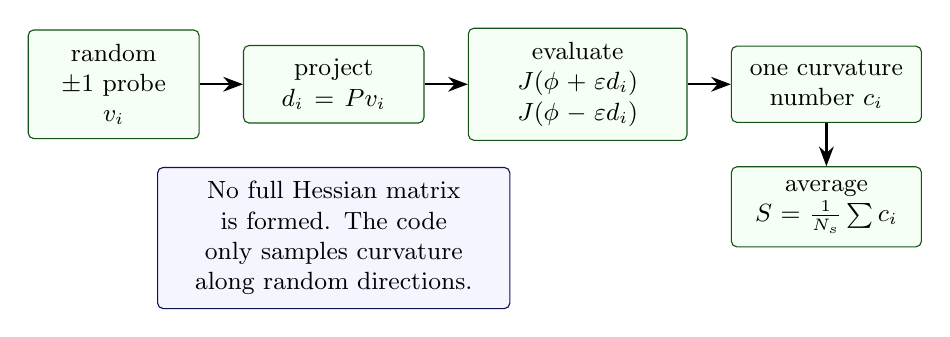
\begin{tikzpicture}[node distance=0.55cm and 0.55cm]
  \node[sharpbox,text width=0.15\textwidth] (a) {random\\$\pm 1$ probe\\$v_i$};
  \node[sharpbox,right=of a,text width=0.16\textwidth] (b) {project\\$d_i=P v_i$};
  \node[sharpbox,right=of b,text width=0.20\textwidth] (c) {evaluate\\$J(\phi+\varepsilon d_i)$\\$J(\phi-\varepsilon d_i)$};
  \node[sharpbox,right=of c,text width=0.17\textwidth] (d) {one curvature\\number $c_i$};
  \node[sharpbox,below=of d,text width=0.17\textwidth] (e) {average\\$S=\frac{1}{N_s}\sum c_i$};
  \node[flowbox,below=of b,text width=0.34\textwidth] (f) {No full Hessian matrix is formed. The code only samples curvature along random directions.};
  \draw[flowarrow] (a) -- (b);
  \draw[flowarrow] (b) -- (c);
  \draw[flowarrow] (c) -- (d);
  \draw[flowarrow] (d) -- (e);
\end{tikzpicture}
\caption{Sharpness is a random average of many one-dimensional curvature measurements.}
\end{figure}

\subsection{Step 1: directional curvature from Taylor expansion}

Take any direction $d$. A second-order Taylor expansion gives
\[
J(\phi+\varepsilon d)
=
J(\phi)
+
\varepsilon \nabla J(\phi)^\top d
+
\frac{\varepsilon^2}{2} d^\top H(\phi) d
+
\mathcal{O}(\varepsilon^3),
\]
and similarly
\[
J(\phi-\varepsilon d)
=
J(\phi)
-
\varepsilon \nabla J(\phi)^\top d
+
\frac{\varepsilon^2}{2} d^\top H(\phi) d
+
\mathcal{O}(\varepsilon^3).
\]

If we add these two expansions, the linear terms cancel:
\[
J(\phi+\varepsilon d)+J(\phi-\varepsilon d)-2J(\phi)
=
\varepsilon^2 d^\top H(\phi)d + \mathcal{O}(\varepsilon^4).
\]

Dividing by $\varepsilon^2$ gives
\[
\frac{J(\phi+\varepsilon d)+J(\phi-\varepsilon d)-2J(\phi)}{\varepsilon^2}
=
d^\top H(\phi)d + \mathcal{O}(\varepsilon^2).
\]

So the symmetric finite difference in the code is estimating the
\emph{directional second derivative} in direction $d$.

\begin{keyidea}
Each probe asks:
\emph{``If I move a little in this direction and a little in the opposite
direction, how bowl-shaped or saddle-shaped is the loss along that line?''}
\end{keyidea}

\subsection{Step 2: from one directional curvature to an average curvature}

Now suppose we do not want the curvature in just one carefully chosen
direction. We want an \emph{average} over many directions. Then we can sample
random probe vectors $v$ and average
\[
v^\top H(\phi) v.
\]

Using random probes is what makes the construction \emph{stochastic}. Instead
of summing over a huge set of directions, which would be expensive, the code
uses a small random set and treats the resulting average as a Monte Carlo
estimate of a larger average.

\subsection{What a Hutchinson-style estimator is, in plain language}

Suppose I ask you to find the average height of every student in a huge
university. One method is to measure every student. That is exact, but slow.
Another method is to sample a few hundred students at random and average those.
That is not exact, but it is much cheaper, and if the sample is chosen well it
can be very accurate.

A Hutchinson-style estimator is the same kind of idea, but for matrix
quantities instead of people.

Here the expensive quantity is the trace of the Hessian, which is the sum of
all diagonal entries:
\[
\tr(H) = H_{11} + H_{22} + \cdots + H_{NN}.
\]

If we had the full Hessian matrix in memory, we could compute that sum
directly. But in this project we usually do \emph{not} have the full Hessian.
We only know how to ask questions of the form
\[
v \mapsto Hv.
\]

So the problem is:
\begin{quote}
How can we estimate a big quantity like $\tr(H)$ using only cheap-ish random
probes, without ever building the full matrix?
\end{quote}

Hutchinson's answer is:
\begin{enumerate}[leftmargin=*]
  \item pick a random vector $v$,
  \item compute the scalar $v^\top H v$,
  \item repeat a few times,
  \item average the results.
\end{enumerate}

That average is the estimator.

The word \emph{style} here just means the repo is using the same basic
mathematical trick, even though it wraps it in finite differences and gauge
projection for this particular physics problem.

\begin{takeaway}
A Hutchinson estimator is just a random-sampling trick for estimating a large
matrix summary, usually a trace, without constructing the whole matrix.
\end{takeaway}

\subsection{Step 3: why this becomes a trace estimator}

For any matrix $H$ and any random vector $v$ with
\[
\E[v v^\top] = I,
\]
we have
\[
\E[v^\top H v]
=
\E[\tr(v^\top H v)]
=
\E[\tr(H v v^\top)]
=
\tr\!\bigl(H\,\E[v v^\top]\bigr)
=
\tr(H).
\]

This is the Hutchinson identity. It says that if the random probes are chosen in
the right unbiased way, then the average quadratic form recovers the trace.

Rademacher probes satisfy exactly this requirement. If the entries of $v$ are
independent and each one is $+1$ or $-1$ with probability $1/2$, then
\[
\E[v_i v_j] =
\begin{cases}
1, & i=j,\\
0, & i\neq j,
\end{cases}
\]
which is exactly the matrix statement
\[
\E[v v^\top] = I.
\]

So for Rademacher probes,
\[
\E[v^\top H v] = \tr(H).
\]

That is why the code samples random $\pm 1$ directions rather than just picking
a few fixed directions by hand.

\subsection{Step 4: what the projector does to the trace}

In the code the direction is not $v$, but $Pv$, where $P$ removes the gauge
subspace. Then the directional curvature becomes
\[
(Pv)^\top H (Pv) = v^\top P^\top H P\, v.
\]

Since the projector used here is orthogonal, $P^\top = P$ and $P^2 = P$, so
the expectation becomes
\[
\E[(Pv)^\top H (Pv)]
=
\tr(P H P).
\]

So the stochastic sharpness quantity is not trying to estimate the trace of the
full Hessian. It is trying to estimate the trace of the Hessian restricted to
the non-gauge subspace.

Here the code applies the estimator not in the full space but in the
gauge-projected subspace, so morally it is estimating the trace of the
\emph{physical} Hessian after removing two known symmetry directions.

\subsection{What this scalar means intuitively}

The trace is the sum of eigenvalues:
\[
\tr(H) = \sum_{k=1}^N \lambda_k.
\]

So the stochastic summary is approximately measuring the \emph{sum of local
curvatures} over all non-gauge directions.

This gives a useful but compressed notion of ``sharpness'':
\begin{itemize}[leftmargin=*]
  \item if many directions are strongly positively curved, the trace tends to
  be large and positive,
  \item if many directions are flat, the trace tends to be small,
  \item if positive and negative curvature coexist, they can cancel.
\end{itemize}

That last point is very important in this repo, because the Phase 13 Hessian
analysis found indefinite saddle structure rather than clean positive-definite
minima.

\subsection{Why we want the trace at all}

The trace is useful because it turns a high-dimensional curvature object into
one understandable number. If the Hessian eigenvalues are
\[
\lambda_1,\lambda_2,\ldots,\lambda_N,
\]
then
\[
\frac{1}{N}\tr(H)
=
\frac{1}{N}\sum_{k=1}^N \lambda_k
\]
is the average curvature per direction.

In optimization language:
\begin{itemize}[leftmargin=*]
  \item a large positive trace means many random directions are bowl-shaped and
  steep,
  \item a smaller trace often means the point sits in a broader, flatter region,
  \item a flatter region is usually more robust to small numerical, physical, or
  modeling perturbations.
\end{itemize}

That is why sharpness regularization penalizes a trace-like quantity. It is a
cheap way to say: ``do not only make the loss small; also prefer solutions where
the loss does not rise too quickly when the phase is nudged.''

\begin{keyidea}
The sharpness path answers a different question:
\emph{``Can I add a cheap curvature penalty to the objective so the optimizer
prefers flatter basins?''}
\end{keyidea}

\section{Why the Gauge Projector Appears in Sharpness}

The Raman cost is invariant under two phase transformations on the input band:
\[
\phi(\omega) \mapsto \phi(\omega) + C + \alpha \omega.
\]

These correspond to:
\begin{itemize}[leftmargin=*]
  \item a constant phase shift,
  \item a linear-in-frequency phase shift, which acts like a time delay.
\end{itemize}

These are gauge directions: they do not change the physical cost. So if the
sharpness estimator probed them directly, it would waste samples measuring
known zero-curvature directions.

The code therefore constructs two orthonormal gauge vectors:
\begin{align*}
u_1 &= \text{constant-on-input-band direction}, \\
u_2 &= \text{centered linear-in-}\omega\text{ direction on the input band},
\end{align*}
and projects by
\[
P(v) = v - \ip{u_1}{v}u_1 - \ip{u_2}{v}u_2.
\]

So all sharpness probes live in the complement of the gauge subspace.

\begin{figure}[htbp]
\centering
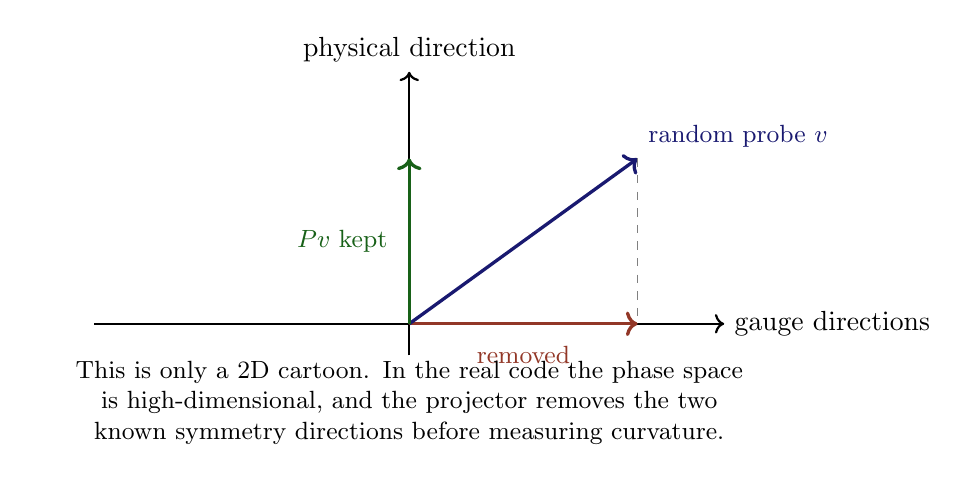
\begin{tikzpicture}[x=1cm,y=1cm]
  \draw[->,thick] (-4,0) -- (4,0) node[right] {gauge directions};
  \draw[->,thick] (0,-0.4) -- (0,3.2) node[above] {physical direction};
  \draw[->,very thick,BrickRed!75!black] (0,0) -- (2.9,0)
    node[midway,below=4pt,font=\small] {removed};
  \draw[->,very thick,MidnightBlue] (0,0) -- (2.9,2.1)
    node[above right,font=\small] {random probe $v$};
  \draw[dashed,gray] (2.9,2.1) -- (2.9,0);
  \draw[->,very thick,ForestGreen!70!black] (0,0) -- (0,2.1)
    node[midway,left=4pt,font=\small] {$Pv$ kept};
  \node[align=center,font=\small,text width=0.78\textwidth] at (0,-1.0)
    {This is only a 2D cartoon. In the real code the phase space is high-dimensional, and the projector removes the two known symmetry directions before measuring curvature.};
\end{tikzpicture}
\caption{Gauge projection removes directions that change phase convention but not the physical Raman cost.}
\end{figure}

\section{How the Gradient of Sharpness is Computed}

The code does not stop at estimating the scalar penalty $S(\phi)$. Since
sharpness is used inside optimization, it also needs $\nabla S(\phi)$.

It computes this by applying the same symmetric finite-difference pattern to
the gradient:
\[
\nabla S(\phi)
\approx
\frac{1}{N_s}
\sum_{i=1}^{N_s}
\frac{
\nabla J(\phi+\varepsilon Pv_i)
+
\nabla J(\phi-\varepsilon Pv_i)
-
2\nabla J(\phi)
}{\varepsilon^2}.
\]

So the sharpness code reuses the existing first-order adjoint gradient oracle.
It does \emph{not} need a true second-order adjoint implementation.

If ``second-order adjoint'' is unfamiliar, you can read that sentence as:
the code avoids building a much more complicated new derivative solver. It
reuses the gradient code it already trusts.

\subsection{What this buys the project}

This is a practical engineering compromise:
\begin{itemize}[leftmargin=*]
  \item full second-order methods would be more exact but much more work,
  \item this estimator is cheaper to implement because it only reuses
  \texttt{cost\_and\_gradient(...)} repeatedly,
  \item the penalty can be dropped directly into L-BFGS as a modified scalar
  objective with a matching gradient.
\end{itemize}

\section{The Actual Sharpness-Aware Objective}

The code minimizes
\[
J_{\mathrm{sharp}}(\phi)
=
J_{\mathrm{reg}}(\phi)
+
\lambda_{\mathrm{sharp}}\, S(\phi),
\]
with gradient
\[
\nabla J_{\mathrm{sharp}}(\phi)
=
\nabla J_{\mathrm{reg}}(\phi)
+
\lambda_{\mathrm{sharp}}\, \nabla S(\phi).
\]

This is then passed to \texttt{Optim.LBFGS()} exactly like a normal objective.

\subsection{Default settings}

The Phase 14 implementation uses defaults:
\begin{itemize}[leftmargin=*]
  \item $\lambda_{\mathrm{sharp}} = 0.1$,
  \item $N_s = 8$ Hutchinson samples,
  \item $\varepsilon = 10^{-3}$ for the sharpness finite difference.
\end{itemize}

By contrast, the Phase 13 HVP/eigenspectrum path uses a smaller finite
difference default,
\[
\varepsilon = 10^{-4},
\]
because it is approximating the Hessian-vector product directly from gradient
differences rather than a trace-like scalar penalty.

\section{When Hessian is Used vs When Sharpness is Used}

\subsection{Hessian is used when the goal is geometry diagnosis}

Use the Hessian path when you want to know:
\begin{itemize}[leftmargin=*]
  \item is the current point a minimum or a saddle,
  \item what are the stiff directions,
  \item what are the negative-curvature escape directions,
  \item how strong is the indefiniteness,
  \item what local second-order structure should guide future methods.
\end{itemize}

Operationally, this happens \emph{after} an optimization run, not inside every
L-BFGS iteration. In the Phase 13 path, it is a post-hoc analysis tool.

The exception is the separate trust-region research optimizer. That path uses
finite-difference HVPs during optimization to build Newton-style steps, but it
still avoids forming the full Hessian matrix.

\subsection{Sharpness is used when the goal is to change the optimizer's
behavior}

Use the sharpness path when you want to say:
\begin{itemize}[leftmargin=*]
  \item do not just find a deep point,
  \item also prefer a locally flatter or more robust point,
  \item do this with the existing first-order infrastructure,
  \item do it during optimization, not only after the fact.
\end{itemize}

Operationally, sharpness is evaluated \emph{inside} the objective at each
optimization iteration.

\begin{takeaway}
\textbf{Hessian} in this repo is primarily for \emph{understanding} the
landscape.

\textbf{Sharpness} in this repo is primarily for \emph{biasing} the optimizer
toward different parts of the landscape.
\end{takeaway}

\section{A Useful Conceptual Comparison}

\begin{center}
\begin{tabular}{p{0.24\linewidth} p{0.33\linewidth} p{0.33\linewidth}}
\toprule
Question & Hessian path & Sharpness path \\
\midrule
Primary role & diagnose local geometry & regularize optimization \\
Main object & $H(\phi)$ or its spectrum & $S(\phi)$, a trace-like scalar \\
Core computation & gradient finite difference for $Hv$ & cost and gradient finite differences over random probes \\
Typical output & eigenvalues, eigenvectors, saddle/minimum verdict; or HVPs for trust-region steps & modified scalar objective and gradient \\
When used & usually post-hoc/offline; also inside the trust-region research optimizer & during sharpness-regularized optimization \\
Space used & full phase space or control space, depending on wrapper & physical phase space with gauge projection \\
\bottomrule
\end{tabular}
\end{center}

\section{An Important Subtlety: Signed Trace Cancellation}

The research notes call out a key issue: the sharpness penalty implemented here
is effectively a \emph{signed} trace-like quantity.

If the Hessian is indefinite, then positive and negative curvature directions
can cancel:
\[
\tr(H) = \sum_i \lambda_i.
\]

So a saddle with large positive and negative eigenvalues could still have a
small trace.

\begin{warningbox}
This means a small sharpness penalty does \emph{not} necessarily mean the basin
is truly flat in every direction. It may mean positive and negative curvature
are canceling.
\end{warningbox}

That is why the repo still keeps the explicit Hessian eigenspectrum machinery.
The eigenspectrum tells you whether the geometry is genuinely flat, strongly
stiff, or saddle-like. The sharpness penalty alone cannot always disambiguate
those cases.

\section{Control-Space vs Physical-Phase-Space Hessians}

In the full-resolution problem, the optimization variable is the physical phase
$\phi$ itself. But in reduced-basis problems the optimization variable may be a
lower-dimensional coefficient vector $x$, with
\[
\phi = \phi(x).
\]

Then the repo can define a Hessian oracle in control space by:
\begin{enumerate}[leftmargin=*]
  \item lifting $x$ to the physical phase $\phi(x)$,
  \item evaluating the physical loss and its gradient with respect to $\phi$,
  \item pulling that gradient back to the control variable.
\end{enumerate}

This matters because the relevant geometry is the geometry of the variables the
optimizer is actually moving, not always the larger full phase space in the
background.

\section{Why the Repo Chose These Implementations}

The design logic is pragmatic:
\begin{enumerate}[leftmargin=*]
  \item The code already had a reliable first-order adjoint gradient.
  \item A second-order adjoint would be a much larger implementation effort.
  \item Finite-difference HVPs are expensive but manageable for diagnostics.
  \item Hutchinson-style sharpness is noisy, but cheap enough to insert into an
  optimizer without rewriting the physics core.
\end{enumerate}

So the codebase uses:
\begin{itemize}[leftmargin=*]
  \item \textbf{Hessian-vector products without forming the full Hessian} for exact-enough local
  geometry analysis and for the separate trust-region research optimizer,
  \item \textbf{stochastic sharpness estimation} for curvature-aware
  regularization during optimization.
\end{itemize}

\section{A Clean Mental Model}

It helps to keep the following hierarchy in mind:

\subsection*{Level 1: Base loss}
\[
J(\phi).
\]
This is the physical or regularized Raman suppression cost.

\subsection*{Level 2: Gradient}
\[
\nabla J(\phi).
\]
This comes from the forward-adjoint method already implemented in the main
optimizer.

\subsection*{Level 3: Hessian-vector product}
\[
H(\phi)v.
\]
This is approximated by finite-differencing the gradient oracle.

\subsection*{Level 4: Hessian eigenspectrum}
\[
\{\lambda_i, q_i\}.
\]
This is extracted from the HVP operator using Arpack, usually only the top and
bottom wings.

\subsection*{Level 5: Sharpness}
\[
S(\phi) \approx \text{average directional curvature over random projected
directions}.
\]
This is a compressed scalar summary of curvature, suitable for use as a
regularizer.

\begin{keyidea}
The Hessian is the full local second-order object.

The sharpness penalty is a deliberately compressed, stochastic summary of that
second-order object.
\end{keyidea}

\section{Final Summary}

\begin{enumerate}[leftmargin=*]
  \item The repository's \textbf{Hessian} machinery is implemented through
  finite-difference Hessian-vector products built from the existing adjoint
  gradient oracle.
  \item Those HVPs are used mainly for \textbf{post-hoc geometry analysis}:
  symmetry checks, Taylor tests, dense small-$N$ verification, and top/bottom
  eigenspectrum extraction with Arpack. A separate trust-region research
  optimizer also uses finite-difference HVPs inside the optimization loop.
  \item The repository's \textbf{sharpness} machinery is a
  \textbf{Hutchinson-style gauge-projected trace estimator} built from repeated
  cost and gradient evaluations.
  \item Sharpness is used \textbf{inside optimization} by minimizing
  \[
  J_{\mathrm{sharp}} = J_{\mathrm{reg}} + \lambda_{\mathrm{sharp}} S.
  \]
  \item Hessian and sharpness are related, but they serve different purposes:
  Hessian explains the local geometry; sharpness biases the optimizer using a
  cheaper summary of that geometry.
  \item Because the implemented sharpness is trace-like and signed, it can hide
  cancellation between positive and negative curvature. That is why the
  explicit Hessian eigenspectrum remains important.
\end{enumerate}

\begin{takeaway}
If you only remember one sentence, remember this:

\textbf{The Hessian code tries to understand the whole local shape of the
landscape, while the sharpness code uses a random-sampling shortcut to boil
part of that shape down to one number that can be used during optimization.}
\end{takeaway}

\end{document}
